\chapter{Проектирование программного обеспечения} \label{ch:ch2}

\section{Типичные архитектуры Fabric ориентированных приложений} \label{sec:ch2:sec1}

Приложения взаимодействуют с сетью Hyperledger Fabric посредством SDK по протоколу gRPC как показано на рисунке \ref{fig:apps_use_sdk}. 
Они обращаются к узлам бизнес сети для вызова и/или запроса чейнкода, чтения данных из блокчейна, регистрируют слушателей событий, а так же выполняют различные административные задачи такие как, запрос и/или изменение конфигурации узлов.

\begin{figure}[ht]
	\centering
	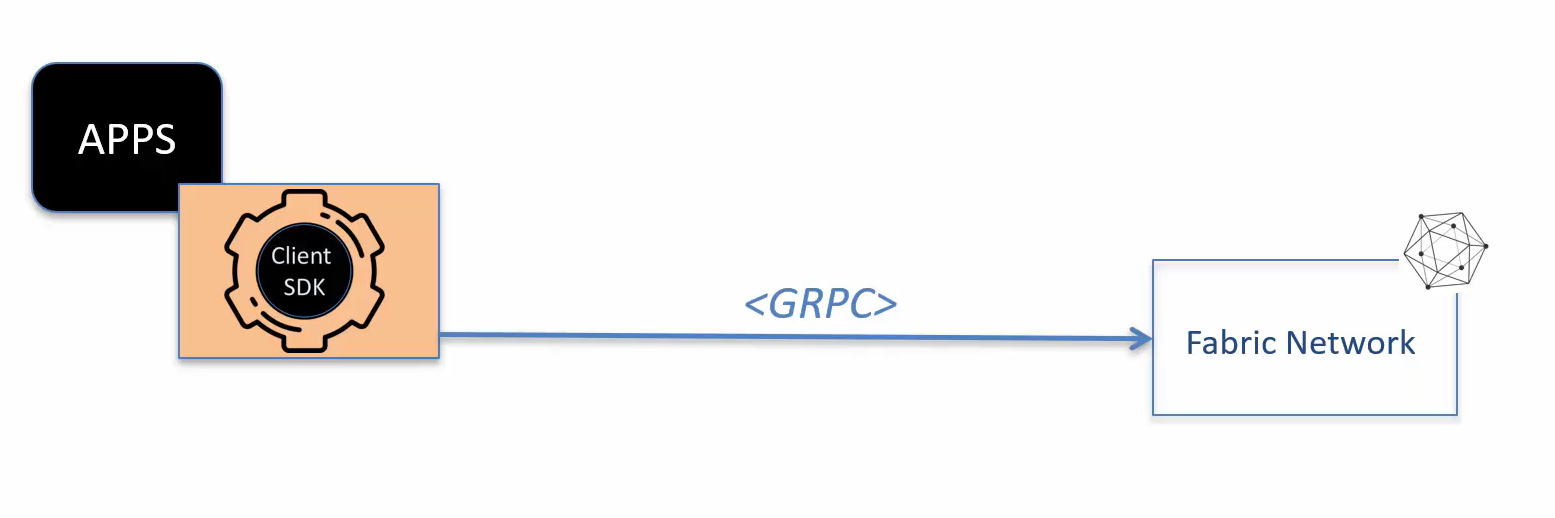
\includegraphics [scale=0.5] {apps_use_sdk}
	\caption{Взаимодействие приложений с Fabric Network}
	\label{fig:apps_use_sdk}
\end{figure}

Как уже упоминалось выше все эти операции осуществляются с помощью Fabric SDK для языков общего назначения. В настоящее время существуют Fabric SDK для языков Java, Go, Python и JavaScript. Так как каждую технологию следует выбирать для тех целей, для которых она подходит лучше всего, то будет справедливым рассмотреть типы Fabric ориентированных приложений. Чаще всего это:

\begin{itemize} 
	\item Графические приложения, позволяющие пользователю выполнять смарт-контракты через графический интерфейс.
	\item Приложения, представляющие отчеты из хранилища данных чейнкода.
	\item Модули интеграции Fabric SDK в уже существующие проекты, для взаимодействия с системами бекенда.
\end{itemize}

При разработки приложения того или иного типа уместно применение соответствующего шаблона архитектуры.
Рассмотрим типичные шаблоны построение Fabric ориентированных приложений.
Настольные приложения - создание и подписание транзакции посходит локально на компьютере пользователя (Рисунок \ref{fig:desktop_apps}). Такой подход является хорошо защищенным, но имеет недостаток в виде дистрибуции приложения. При внесении правок в приложение, конечный пользователь вынужден в ручную устанавливать обновления на свой компьютер.
\begin{figure}[ht]
	\centering
	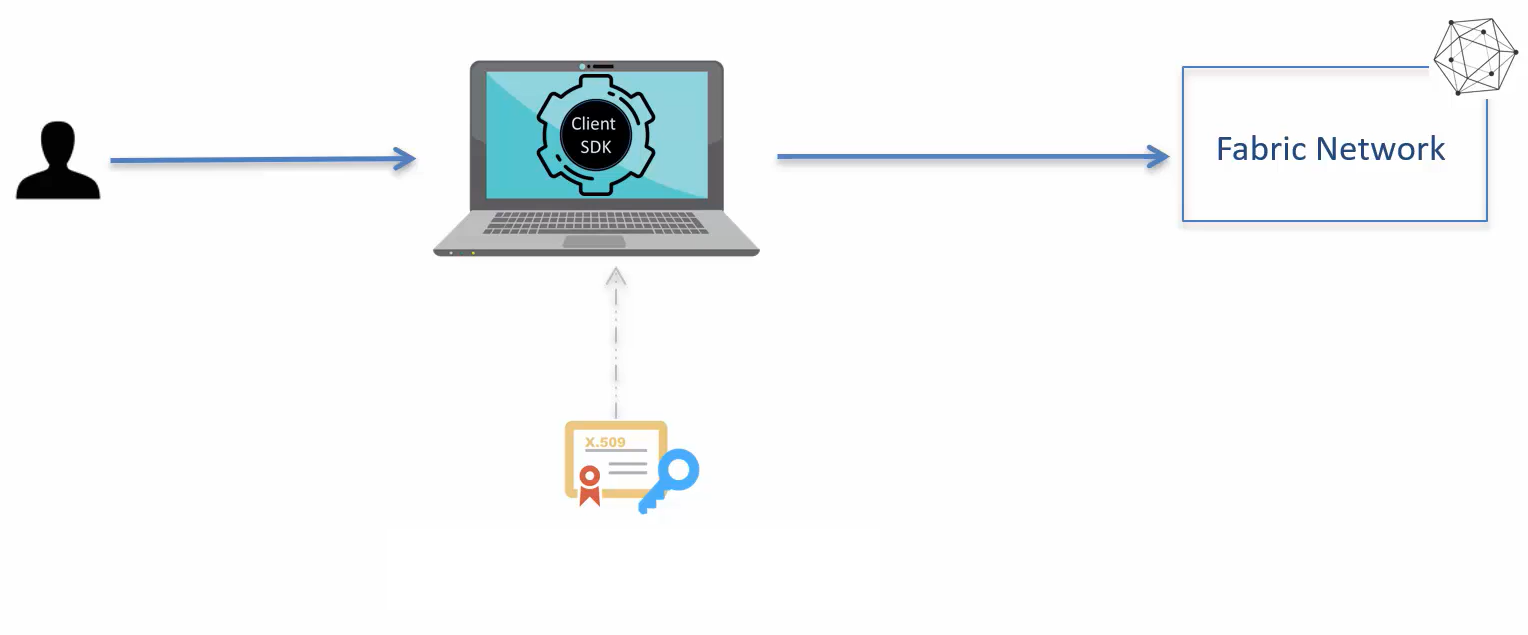
\includegraphics [scale=0.5] {desktop_apps}
	\caption{Настольные приложения, использующие Fabric SDK}
	\label{fig:desktop_apps}
\end{figure}

Обработка транзакций в сети Fabric приводит к возникновению различных событий, которые могут потребляется приложениями. События могут предоставятся клиента посредством некого брокера сообщений (например, Kafka), или же посредством REST-API. При получении определенного события клиентское приложение соответствующим образом обрабатывает его(например, обновляет свои бекенд системы). Так как события инициируются и обрабатываются в режиме реального времени, такой подход широко используется для создания инфопанелей и отчетов в режиме реального времени. Схематично данный шаблон предоставлен на рисунке \ref{fig:event_hub}.

\begin{figure}[ht]
	\centering
	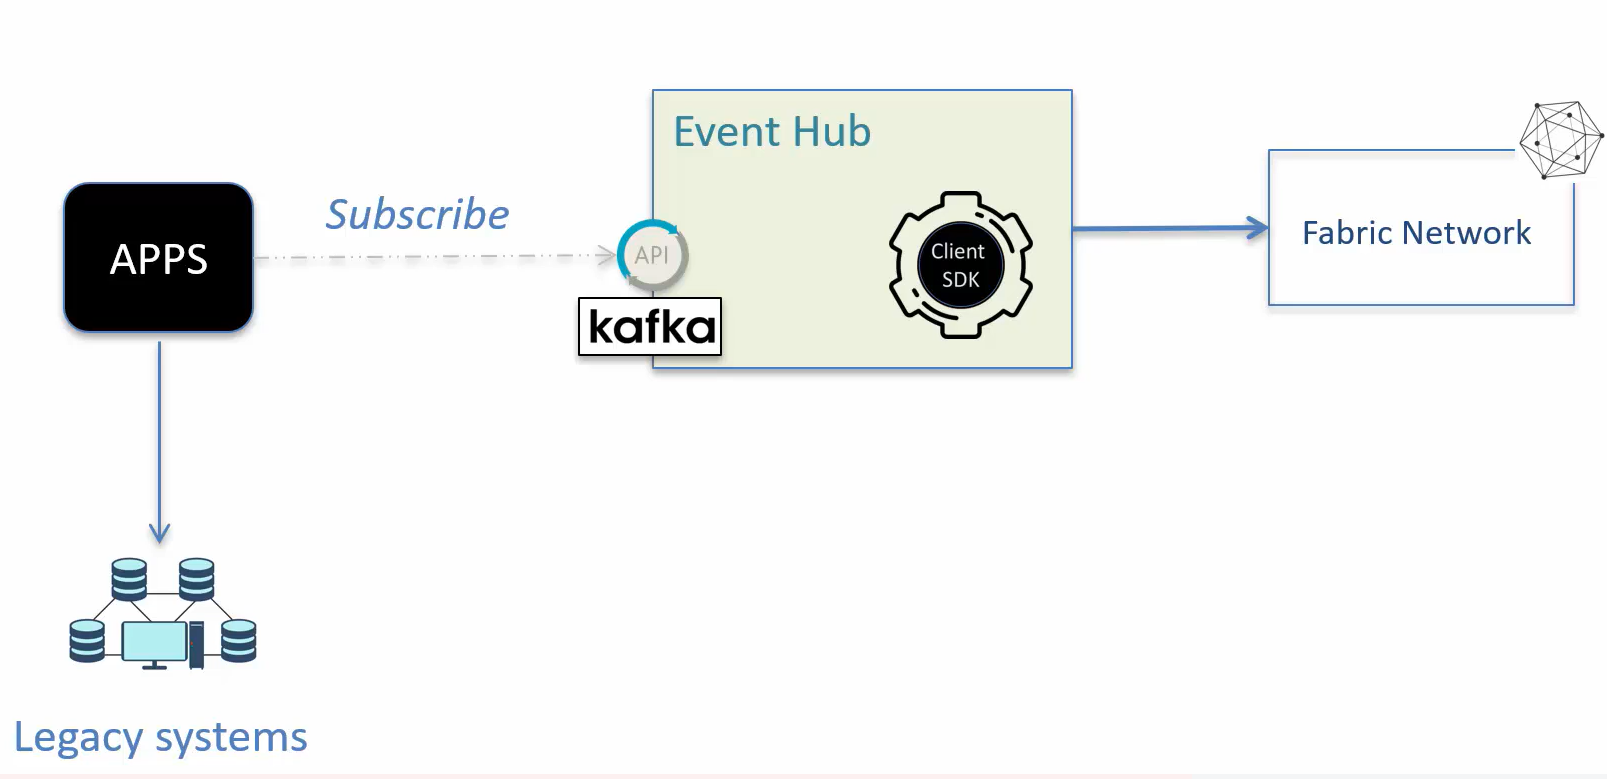
\includegraphics [scale=0.5] {event_hub}
	\caption{Архитектура <<Event Hub>>}
	\label{fig:event_hub}
\end{figure}
А также Fabric SDK может быть использована для создания различных утилит командной строки. Эти утилиты используется администраторами бизнес сети Hyperledger Fabric для осуществления различных административных задач (Рисунок \ref{fig:admin_cli}).
\begin{figure}[ht]
	\centering
	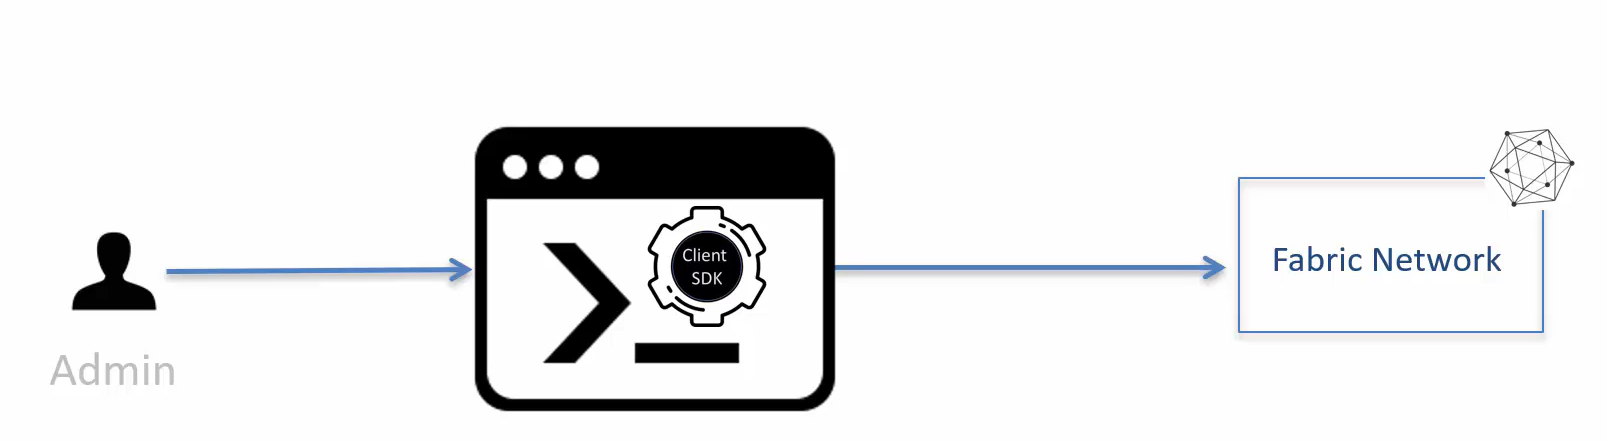
\includegraphics [scale=0.5] {admin_cli}
	\caption{Утилиты командной строки}
	\label{fig:admin_cli}
\end{figure}

Ещё один широк распространенный подход к построению Fabric ориентированных приложений - использование связующего программного обеспечения, ориентированное на обработку сообщений \cite{middleware} (англ. message-oriented middleware). Это ПО использует Fabric SDK, и обеспечивает связь среды выполнения Fabric с клиентским приложением. Middleware предоставляет API, обращаясь к которому клиентские приложения взаимодействуют с бизнес сетью. При этом тип клиентского приложения может быть любым(настольное, мобильное, веб и д.р.). Cхема такой архитектуры представлена на рисунке \ref{fig:middleware}.

\begin{figure}[ht]
	\centering
	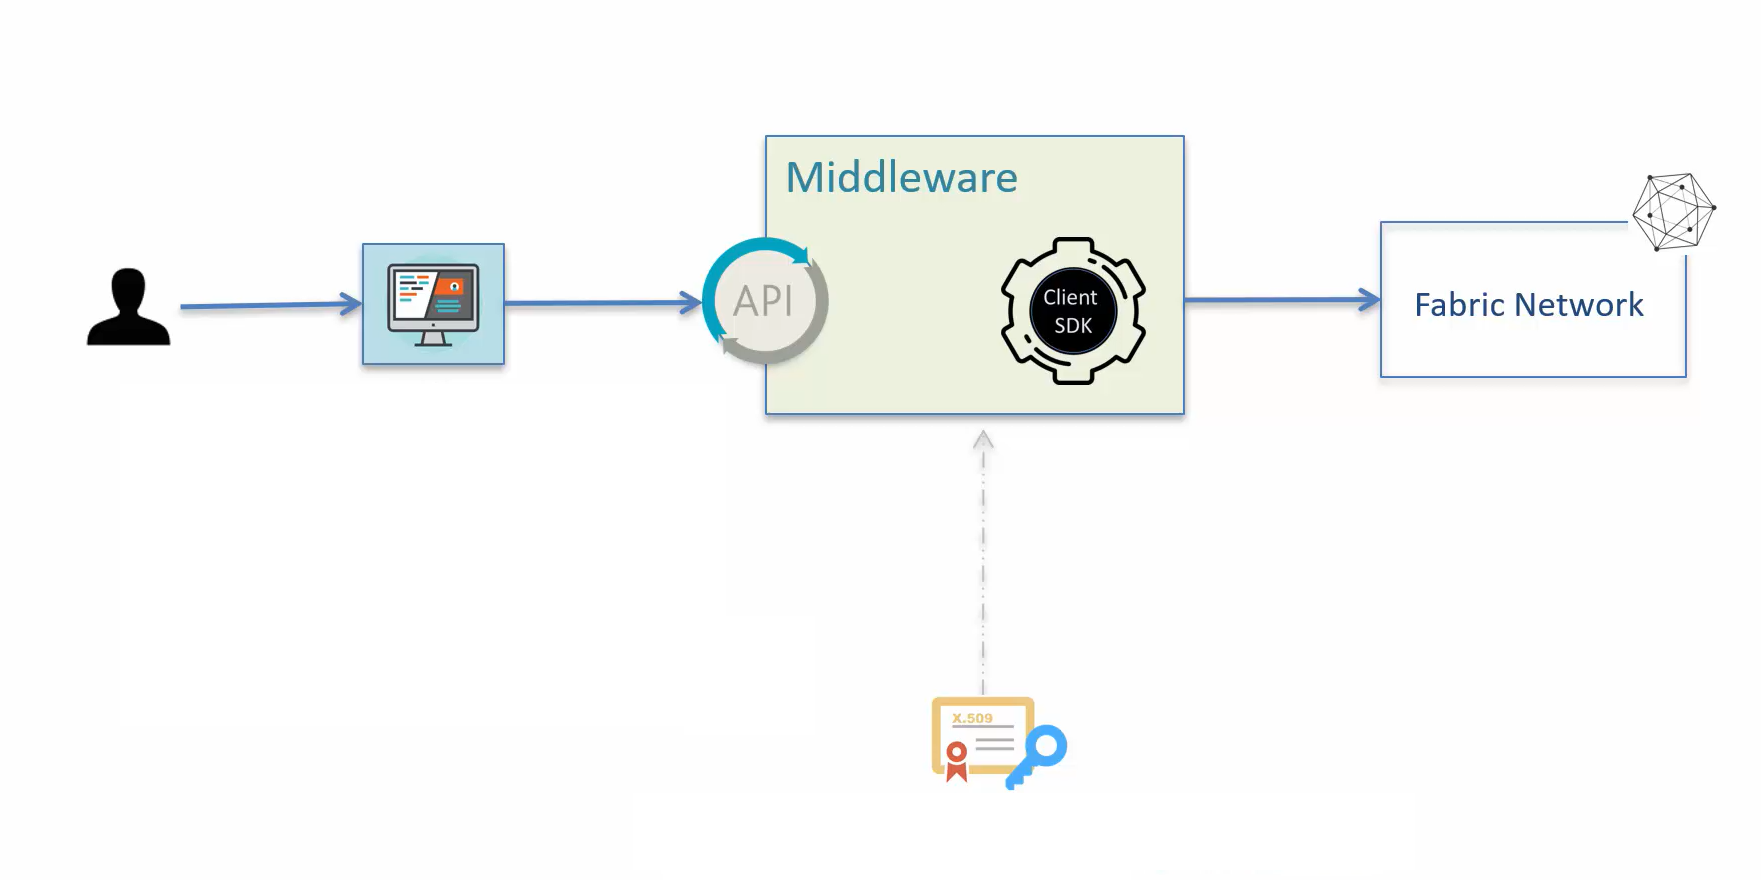
\includegraphics [scale=0.5] {middleware}
	\caption{Архитектура со связующим ПО}
	\label{fig:middleware}
\end{figure}
Но при реализации такого подход возникает ряд вопросов, и первый из них где управлять ключами и сертификатами пользователей? Один из вариантов - управлять ими на стороне middleware. Однако в этом случае пользователи должны доверять хосту middleware, т.к. их приватные ключи оседают на его стороне. Однако в некоторых случаях пользователи могут не доверять организации, осуществляющей хостинг middleware. В таких случаях необходимо закладывать логику работы с приватными ключами и сертификатами на стороне клиентского приложения. Очевидно, что такой подход является более защищенным, однако он так же имеет недостаток в виде увлечения сложности приложения. А также в этом случае нарушается принцип единственной ответственности (SRP). \cite{solid}


\section{Архитектура ПО} \label{sec:ch2/sec2}
В \ref{sec:ch2:sec1} мы рассмотрели типичные архитектуры  Fabric ориентированных приложений. В данной работе выбор пал на архитектуру со связующим ПО с инкапсуляцией логики работы с сертификатами пользователей на стороне связующего ПО. В представленных в работе сценариях отношение между отдельными элементами доверительные, поэтому недостаток данного подхода не создает проблем. К очевидными плюсам данной архитектуры можно, также отнести легкую замену графического клиентского приложения, т.к. ему неизвестно существование бизнес сети, оно работает исключительно со связующим ПО по технологии RPC. \cite{grpc}
На рисунке \ref{fig:sys_architecture} представлена схема архитектуры разработанного приложения.
\begin{figure}[ht]
	\centering
	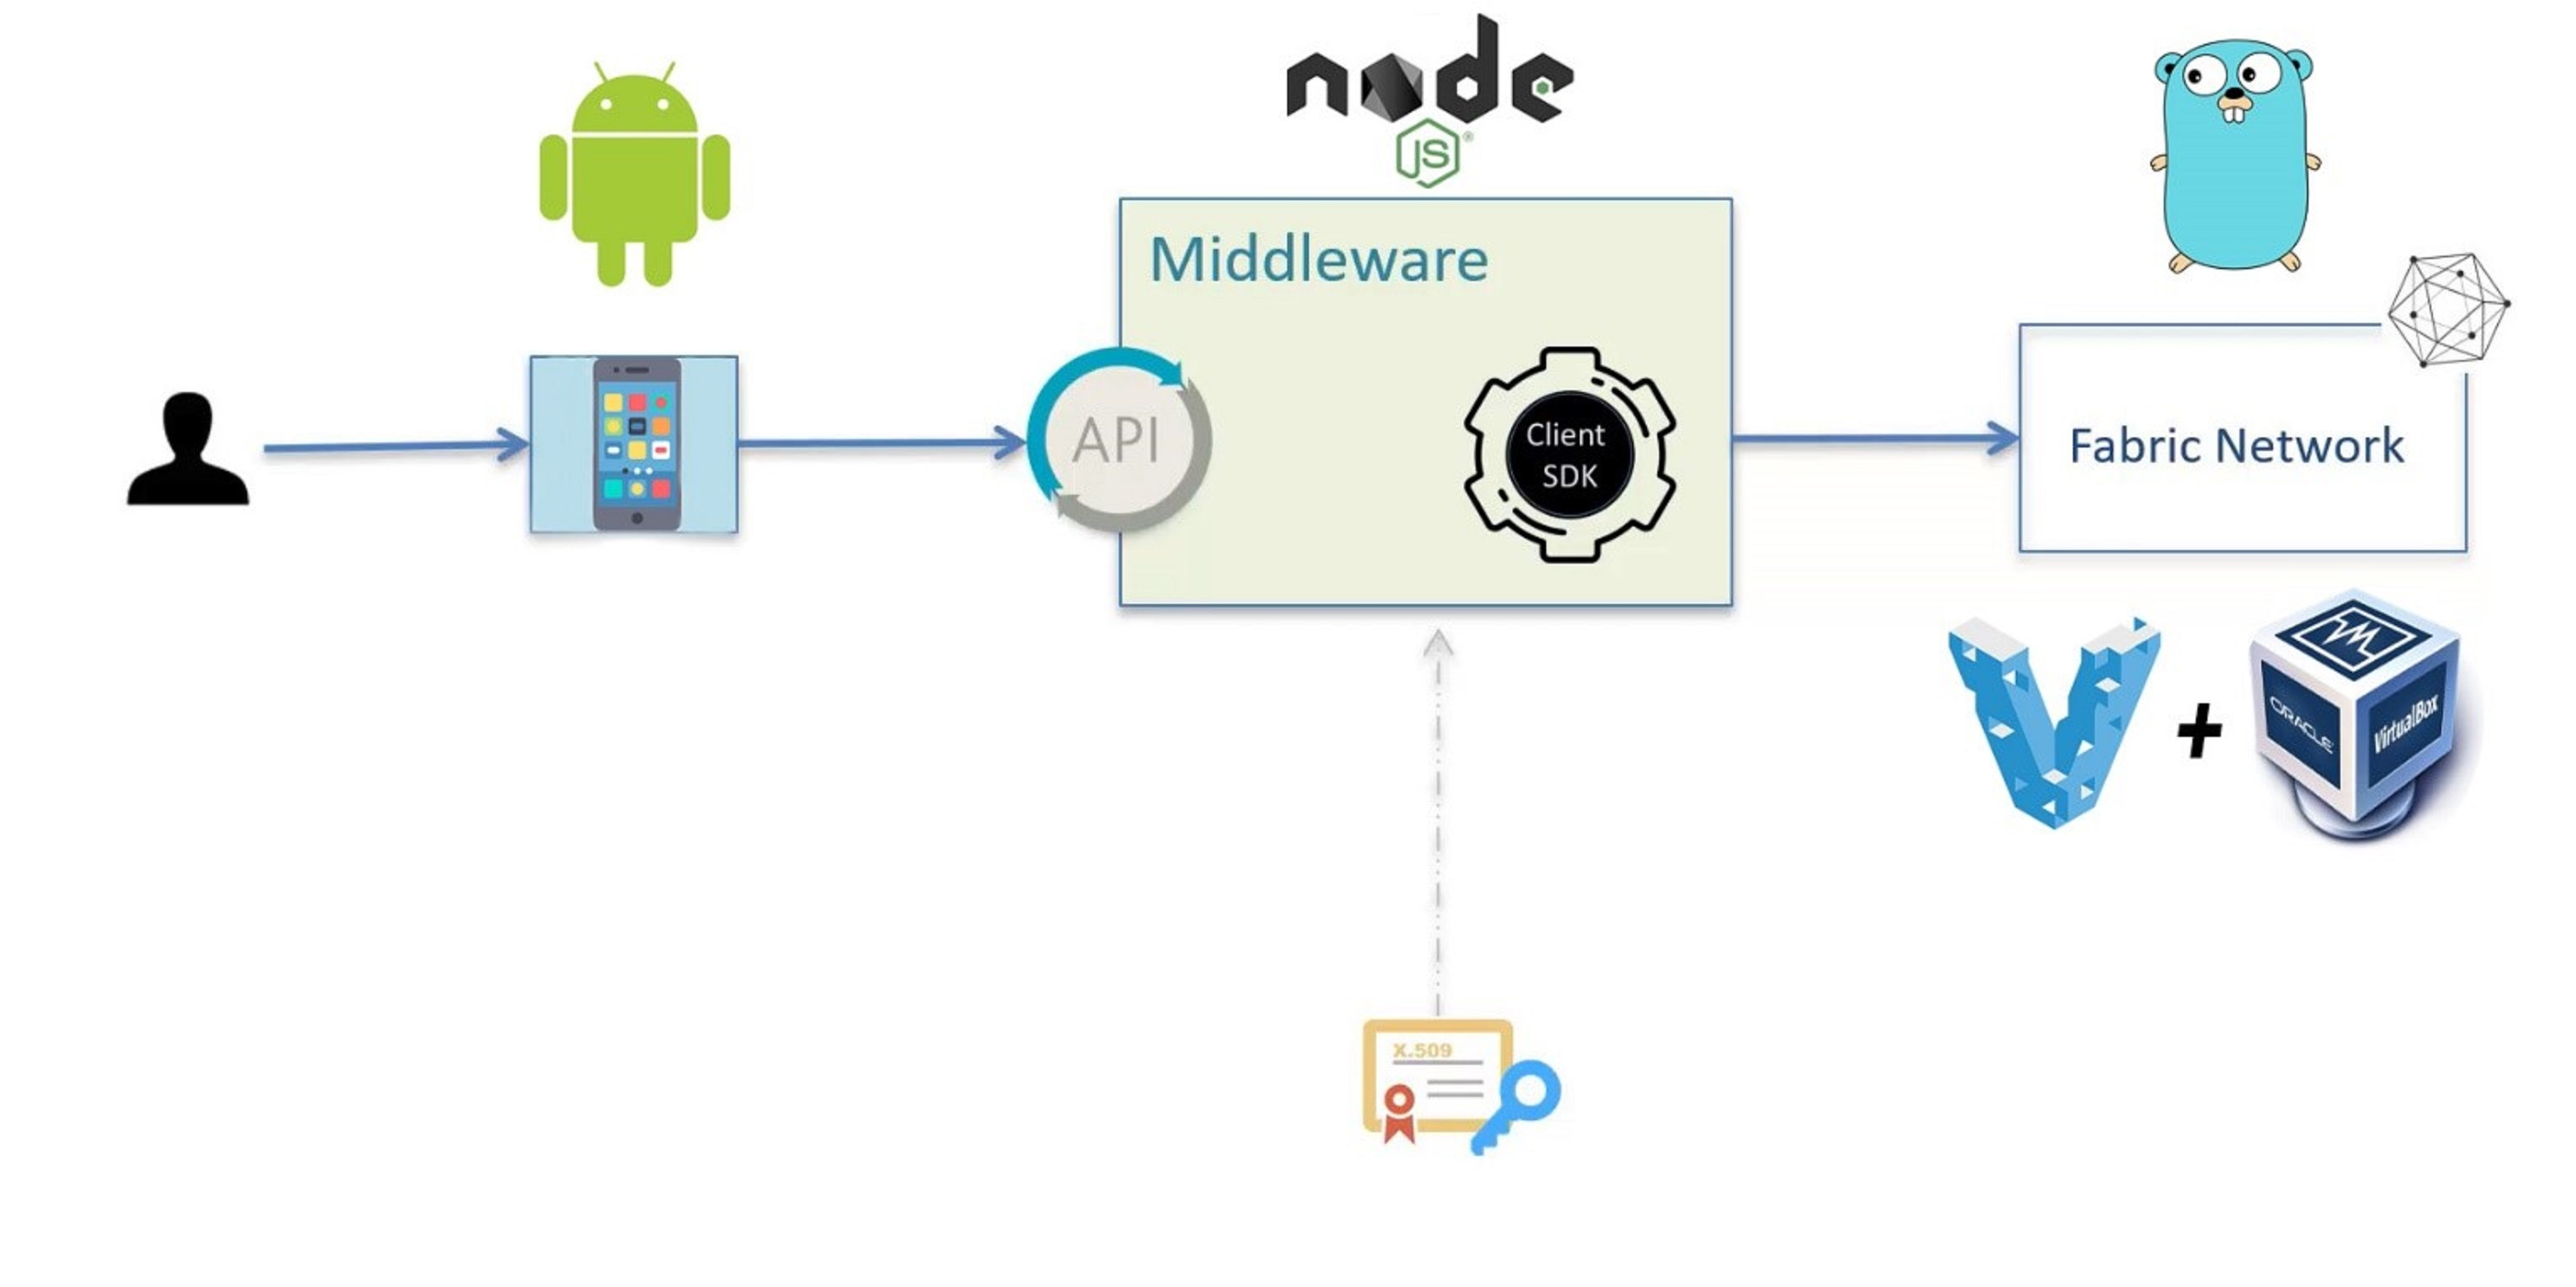
\includegraphics [scale=0.5] {sys_architecture}
	\caption{Архитектура разработанного приложения.}
	\label{fig:sys_architecture}
\end{figure}

\section{Выбор инструментов и технологий} \label{sec:ch2:sec3}
\subsection{Развертка бизнес сети} \label{subsec:ch2/sec3/subsec1}

Для разработки и отладки смарт контрактов требуется их разворачивание на пирах бизнес сети. Проще всего разворачивать такую тестовую сеть на виртуальной машине, на которую пред установлено  все необходимое программное обеспечение, а именно:
\begin{itemize}
	\item Docker и Docker Compose \cite{docker};
	\item Компилятор и стандартные библиотеки языка Go \cite{golang};
	\item Менеджер пакетов языка Go govendor \cite{govendor}; 
	\item Бинарные файлы Hyperledger Fabric \cite{fabric-bins};
	\item Пакеты Shim и Shimtest \cite{shim-go}.
\end{itemize}

На это виртуальной машине запускаются docker-контейнеры, представляющие из себя различные элементы бизнес сети Fabric (orderers, endorser, peers). Таким образом, образуются тестовая бизнес сеть внутри которой легко разрабатывать, отлаживать и тестировать смарт контракты. Запуск виртуальной машины и остановка среды разработки происходит с помощью Oracle Virtual Box \cite{oracle-vbox-site} и Vagrant \cite{vagrant-site}.

Отдельно внимания заслуживает такой инструмент как Vagrant, поскольку он сильно облегчает развертку среды разработки. 
Vagrant - это программное обеспечение с открытым исходным кодом, предназначенное для построения и поддержки виртуальных сред разработки на основе, например, Virtual Box, Hyper-V, Docker контейнеров. Основная задача этого инструмента - упростить конфигурационное управление (англ.software configuration management, SCM) \cite{scm} и улучшить продуктивность разработчика. 
Создание виртуальной машины происходит при помощи файла конфигурации Vagrantfile, содержимое которого представлено в листинге \ref{lst:vagrantfile}.

\begin{lstlisting}[caption={Конфигурация виртуальной машины: Vagrantfile},label={lst:vagrantfile},language=Ruby]
	Vagrant.configure("2") do |config|
	config.vm.box = "bento/ubuntu-18.04"
	
	# Проброс портов
	# Для CouchDB
	config.vm.network "forwarded_port", guest: 5984, host: 5984
	# Для Hyperledger Explorer
	config.vm.network "forwarded_port", guest: 8080, host: 8080
	# Для Orderer контейнера
	config.vm.network "forwarded_port", guest: 7050, host: 7050
	
	# Для Peer контейнеров
	config.vm.network "forwarded_port", guest: 7052, host: 7052
	config.vm.network "forwarded_port", guest: 9052, host: 9052
	config.vm.network "forwarded_port", guest: 7051, host: 7051
	config.vm.network "forwarded_port", guest: 8052, host: 8052
	config.vm.network "forwarded_port", guest: 9051, host: 9051
	config.vm.network "forwarded_port", guest: 8051, host: 8051
	config.vm.provision "shell", inline:  $script /home/vagrant/app/sdk/vagrant_node_modules
	end
\end{lstlisting}


После создание виртуальной машины, управление ею осуществляется при помощи выполнения следующих команд в директории с Vagrantfile:
\begin{itemize}
	\item \textit{vagrant up} - запуск машины с заданной конфигурацией;
	\item \textit{vagrant ssh} - подключение к виртуальной машине посредством сетевого протокола SSH;
	\item \textit{vagrant halt} - остановка виртуальной машины;
	\item \textit{vagrant destroy} - удаление виртуальной машины.
\end{itemize}
Таким образом, мы имеем удобную среду для разработки, отладки и тестирования смарт контрактов.

\subsection{Смарт контракты} \label{subsec:ch2/sec3/subsec2}

Написание смарт контрактов осуществляется на языках программирования общего назначения, таких как JavaScript, Java и Go. В данной работы смарт контракты написаны на языке Go - разработанным компанией Google языке со статической типизацией. Синтаксически схож с  языком С, однако имеет преимущества перед ним в виде безопасного доступа к памяти, сборкой мусора и удобством реализации параллельных вычислений.

Смарт контракт на языке Go представляет из себя реализацию интерфейса Chaincode из пакета github.com/hyperledger/fabric-chaincode-go/shim.
 
\begin{lstlisting}[caption={Интерфейс Chaincode},label={lst:ichaincode},language=Go]
 type Chaincode interface {
 	
 	Init(stub ChaincodeStubInterface) pb.Response
 
 	Invoke(stub ChaincodeStubInterface) pb.Response
 	
 }
\end{lstlisting}
 
Как видно из листинга \ref{lst:ichaincode} необходимо реализовать две функции: 

\begin{enumerate}
	\item Init - в ней закладывается логика инициализации внутреннего состояния смарт контракта. Она вызывается в момент создания контейнера смарт контракта.
	\item Invoke - содержит бизнес логику смарт контракта
\end{enumerate}

Помимо этих двух функций необходимо зарегистрировать экземпляр  смарт контракт в среде выполнения Fabric. Кога клиентское приложение обращается к сети Fabric, оно передает ей название смарт контракта, название функции смарт котракта и набор параметров. Среда выполнения сопоставляет переданное название смарт контракта с экземплярами смарт контрактов зарегистрированными в среде выполнения и делегирует обращение клиента соответствующей функции соответствующего смарт контракта. Регистрация смарт контракта осуществляется в главной функции Go (main) посредством вызова функции shim.Start с передачей ей экземпляра смарт контракта в качестве параметра. Таким образом шаблон типичного смарт контракта на языке Go имеет вид представленный в листинге \ref{lst:chaincode-impl}.

\begin{lstlisting}[caption={Реализация Chaincode},label={lst:chaincode-impl},language=Go]
	package main
	
	import (
		pb "github.com/hyperledger/fabric-protos-go/peer"
		"github.com/hyperledger/fabric-chaincode-go/shim"
		"fmt"
	)
	
	// SampleSmartContract - пример смарт контракта
	type SampleSmartContract struct {}

	func (ssc *SampleSmartContract) Init(stub shim.ChaincodeStubInterface) pb.Response {
		// логика инициализации
	}
	
	func (ssc *SampleSmartContract) Invoke(stub shim.ChaincodeStubInterface) pb.Response {
		// бизнес логика
	}
	
	func main() {
		e := shim.Start(new(SampleSmartContract))
		if e != nil {
			fmt.Printf("Ошибка регистрации смарт-контракта: %s", e)
		}
	}
\end{lstlisting}


Каждый раз при обращении клиента к смарт контракту среда выполнения Fabric создает экземпляр shim.ChaincodeStubInterface и делегирует вызов соответствующей функции смарт контракта с созданным экземпляром в качестве параметра. В листинге \ref{lst:chaincode-impl}, как формальный параметр интерфейса функций Chaincode фигурирует переменная stub типа shim.ChaincodeStubInterface. Путем манипулирования этим параметром смарт контракт взаимодействует с бизнес сетью Fabric. Stub представляет различные функции, одной из которых является извлечения информации о запросе клиента (название функции и параметров). Таким образом, реализация функции Invoke сводится к классической множественной диспетчеризации \cite{solid}, как показано в листинге \ref{lst:invoke-impl}.

\begin{lstlisting}[caption={Шаблон реализации Chaincode.Invoke},label={lst:invoke-impl},language=Go]
	...
	
	func (t *SampleSmartContract) Invoke(stub shim.ChaincodeStubInterface) pb.Response {
		...
		f, params := stub.GetFunctionAndParameters()
		
		fmt.Println("Вызов функции Invoke : ", f, " параметры=", params)
		
		switch {
			case f == "funcA":
			return processA(stub, params)
			case f == "funcB":
			return processB(stub, params)
			case f == "funcC":
			return processC(stub, params)
			...
		}
		...
	}
	
	...
\end{lstlisting}

\subsection{REST-сервер} \label{subsec:ch2/sec3/subsec3}

Для обеспечения связи клиентского приложение со связующим ПО в качестве методологии RPC был выбран REST (Representational State Transfer — передача состояния представления)\cite{restful} Философия этого подхода заключается в том, что приложения моделируются как набор ресурсов, с которыми клиенты могут взаимодействовать (считывать данные, обновлять, удалять и т.д.). В наше время построение приложений с помощью архитектурного стиля REST вкупе с HTTP и JSON\cite{json} стало фактическим стандартом для создания микросервисов.

Как уже упоминалось в \ref{sec:ch2:sec1}, Fabric SDK существует для нескольких языков программирования общего назначения, среди которых присутствует JavaScript \cite{pure-js}.

\subsubsection{Защита сервера} \label{subsubsec:ch2/sec3/subsec4/subsubsec1}
Слабым местом в представленной схеме \ref{fig:sys_architecture} является линия взаимодействия клиентского приложения со связующим ПО. Оно подвержено различным атакам, таким например как <<Человек посередине>> или MITM (англ. Man In The Middle) \cite{mitm-site}. Для предотвращения таких атак клиент и сервер взаимодействуют по защищенному транспортному протоколу HTTPS, основанному на криптографическом протоколе   SSL, призванным обеспечить безопасность передачи данных по сети. 
В SSL используется ассиметричный алгоритм шифрования. Это означает что, для шифрования используется открытый ключ, а для дешифрования используется приватный ключ. Т.е. всего два ключа для каждой из сторон. Схема передачи данных для такого случая представлена на рисунке \ref{fig:ssl_scheme}

\begin{figure}[ht]
	\centering
	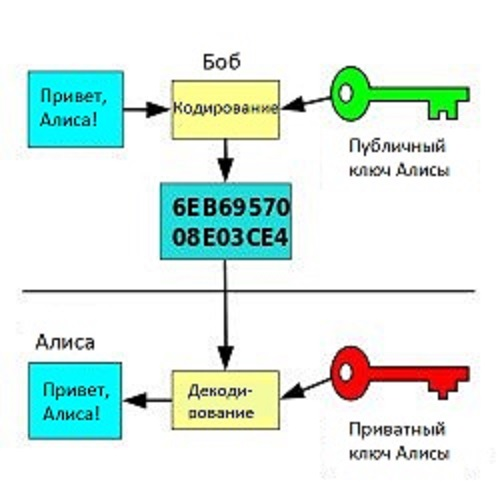
\includegraphics [scale=1.0] {ssl_scheme_rus}
	\caption{Передача данных с использованием ассиметричного алгоритма шифрования.}
	\label{fig:ssl_scheme}
\end{figure}

Хотя использование HTTPS не гарантирует всеобъемлющую безопасность, оно создает неимоверные трудности для злоумышленников.
\subsubsection{JSON Web Token} \label{subsubsec:ch2/sec3/subsec4/subsubsec2}
В наше время разработчики предпочитают использовать аутентификацию основанную на токенах (Token-Based Authentication), вместо привычных сессий. Подход с токенами имеет множество преимуществ перед подходом с сессиями. В разработанной системы для коммуникации клиентского приложения с серверной частью  используется JWT\cite{jwt-site} (Json Web Token). После аутентификации клиентского приложения через защищенный канал SSL, ему выдается сгенерированный JWT, который помещается в заголовке API запроса, каждый раз при обращении к API сервера, требующем идентификации личности пользователя, использующего клиентское приложение. Типовая схема работы описанного подхода представлена на рисунке \ref{fig:jwt_scheme}.

\begin{figure}[ht]
	\centering
	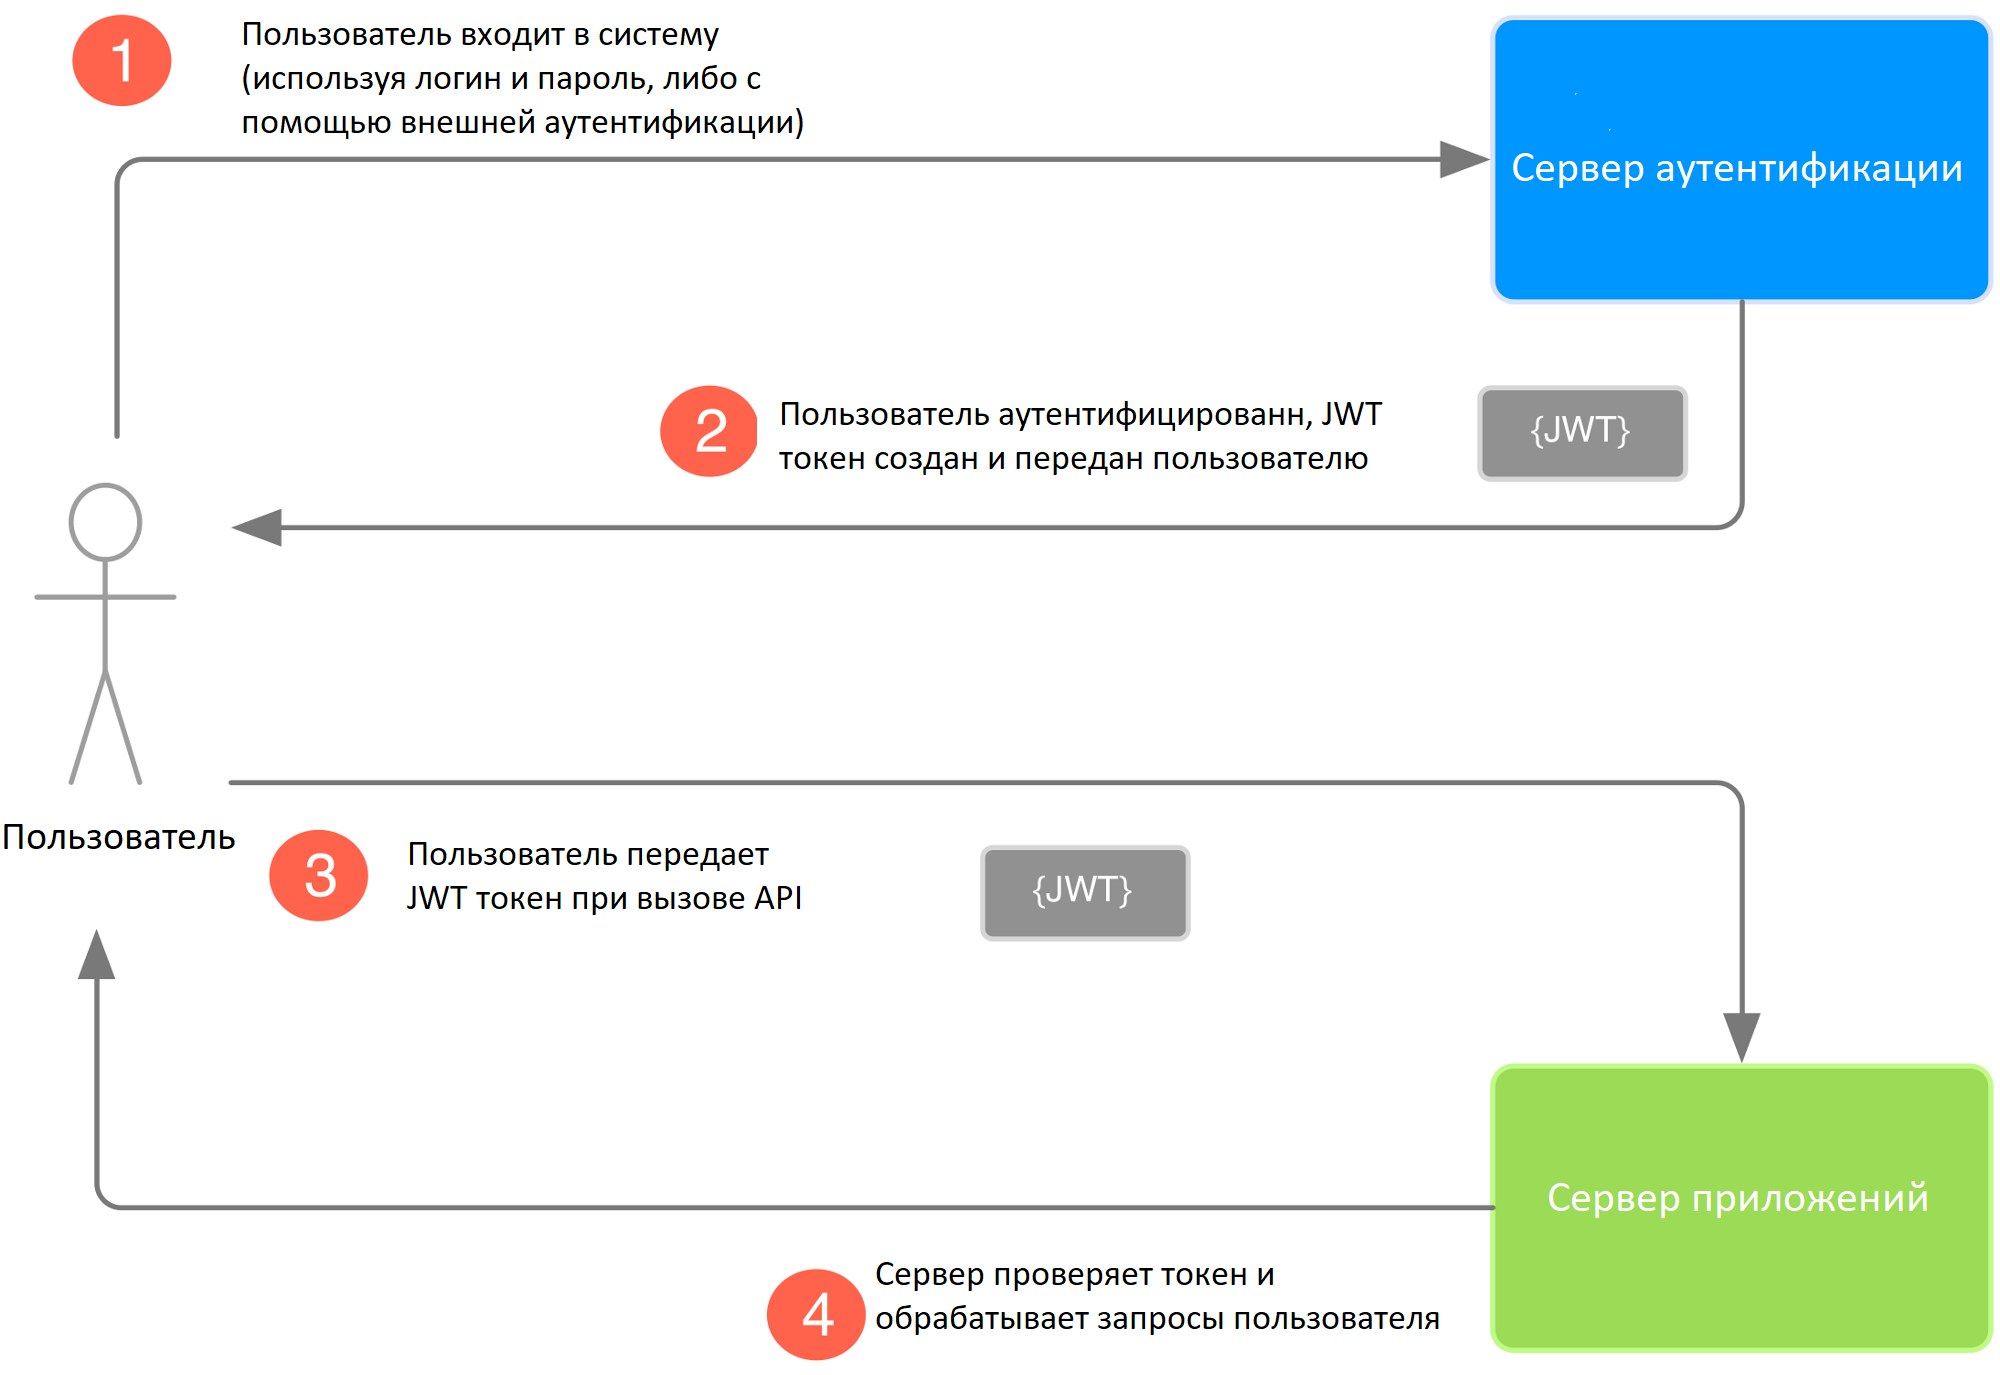
\includegraphics [scale=0.4] {jwt_scheme_rus}
	\caption{Схема работы с JWT.}
	\label{fig:jwt_scheme}
\end{figure}

Структурно JWT токен состоит из трех частей: заголовка, данных и подписи. Заголовок и данные представлены в формате JSON объектов. В то время как подпись генерируется на основе первых двух частей с применением определенного алгоритма шифрования, указанного в заголовке токена. Примеры заголовка и данных приведены в листингах \ref{lst:jwt-header-sample} и \ref{lst:jwt-payload-sample}.

\begin{lstlisting}[caption={Пример JWT загаловка},label={lst:jwt-header-sample},language=JavaScript]
{
	"alg": "HS512",
	"typ": "JWT"
}
\end{lstlisting}

\begin{lstlisting}[caption={Пример JWT данных},label={lst:jwt-payload-sample},language=JavaScript]
	{
		"sub": "12345",
		"name": "John Gold",
		"admin": true
	}
\end{lstlisting}

JWT токен сериализуется к компактном ввиду путем применения алгоритма кодирования Base64-URL к заголовку и данным, после чего происходит конкатенация заголовка, данных и подписи с разделением этих элементов точками.
Сгенерированный JWT токен для примеров из листингов \ref{lst:jwt-header-sample} и \ref{lst:jwt-payload-sample} будет иметь вид представленный в листинге \ref{lst:jwt-token-sample} (для наглядности были добавлены поясняющие комментарии и переводы строк, но в реально приложении JWT токен является одной строкой без пробелов).
\begin{lstlisting}[caption={Пример сгенерированного JWT токена},label={lst:jwt-token-sample},language=JavaScript]
# base64UrlEncode(header)
eyJhbGciOiJIUzUxMiIsInR5cCI6IkpXVCJ9.
# base64UrlEncode(payload)
eyJzdWIiOiIxMjM0NSIsIm5hbWUiOiJKb2huIEdvbGQiLCJhZG1pbiI6dHJ1ZX0K.
# signature
LIHjWCBORSWMEibq-tnT8ue_deUqZx1K0XxCOXZRrBI

\end{lstlisting}

% .
%TODO:  JWT does not secure communication transport over non-secured connection like HTTP. JWT is mainly an authentication system and should only be used with HTTPS but JWT does not increase the security level of HTTPS. Maybe your inverted question would make more sense 

%https://stackoverflow.com/questions/50429209/https-or-jwt-for-authentication/50429642
\subsection{Клиентское приложение}
 \label{subsec:ch2/sec3/subsec4}
 
Выбор мобильного приложения в качестве клиентского в данном случае определяет язык программирования для его разработки.
Под управлением операционной системы Android работает подавляющее число мобильных устройств. Так как предполагается эксплуатация ПО в среде Android, то для реализации ПО в работы выбран язык Java.
 
Этот модуль является  клиентской стороной пользовательского интерфейса к бизнес сети Fabric.  Используя это приложение,  установленное  на смартфон,  клиент  может создавать, подписывать и просматривать документы своей организации.  Мобильное приложение посылает REST API запросы и получает ответы в формате JSON. Эти ответы  используются  для  предоставления  данных  через  понятные  пользователю интерфейсы.

\subsubsection{Пользовательские сценарии}
 \label{subsec:ch2/sec3/subsec4/subsubsec1}
Функциональные требования к клиентскому приложению следующие:
\begin{itemize}
	\item Создание  нового  документа.  Данный  сценарий  описывает  поведение пользователя,  включающее  в  себя  заполнение  полей  документа,  включая  выбор типа документа;
	\item Просмотр  своих  документов.  Пользователь  видит,  созданные  им  ранее 
	документы, их статусы;
	\item Подписание документа. Пользователь перед подписанием может просмотреть 
	всю  необходимую  информацию  о  документе,  а  затем  принять  решение  о 
	дальнейшем действии: подписать, отклонить пс комментарием.
\end{itemize}
Все действия пользователя выполняются через графический интерфейс мобильного приложения. Удобнее всего представить работу приложения с точки зрения пользователя в виде UML диаграммы вариантов использования ПО. Соответствующие диаграммы приведены на рисунках \ref{fig:user-scenario-first}-\ref{fig:user-scenario-last}.

\begin{figure}[H]
	\centering
	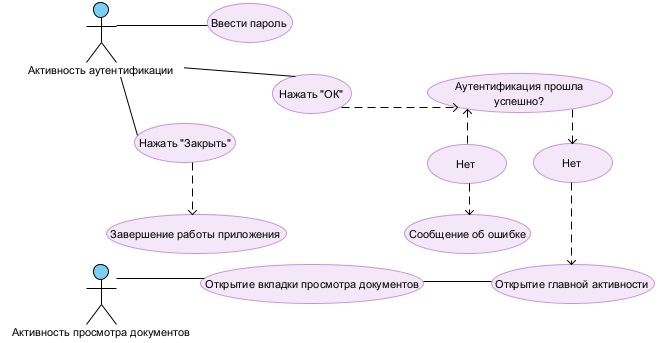
\includegraphics [scale=1.2] {AuthDiagram}
	\caption{Аутентификация пользователя.}
	\label{fig:user-scenario-first}
\end{figure}
\begin{figure}[H]
	\centering
	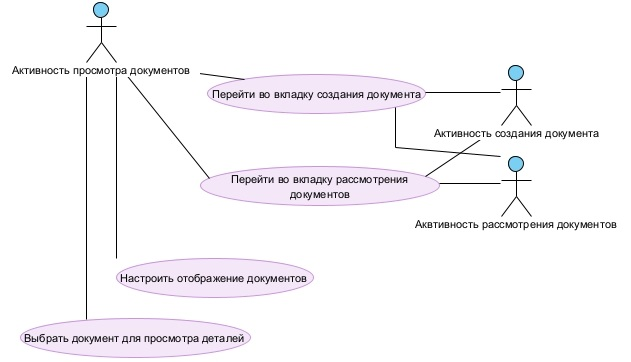
\includegraphics [scale=1.2] {MainDiagram}
	\caption{Просмотр списка документов.}
	\label{fig:user-scenario-view-docs}
\end{figure}
\begin{figure}[H]
	\centering
	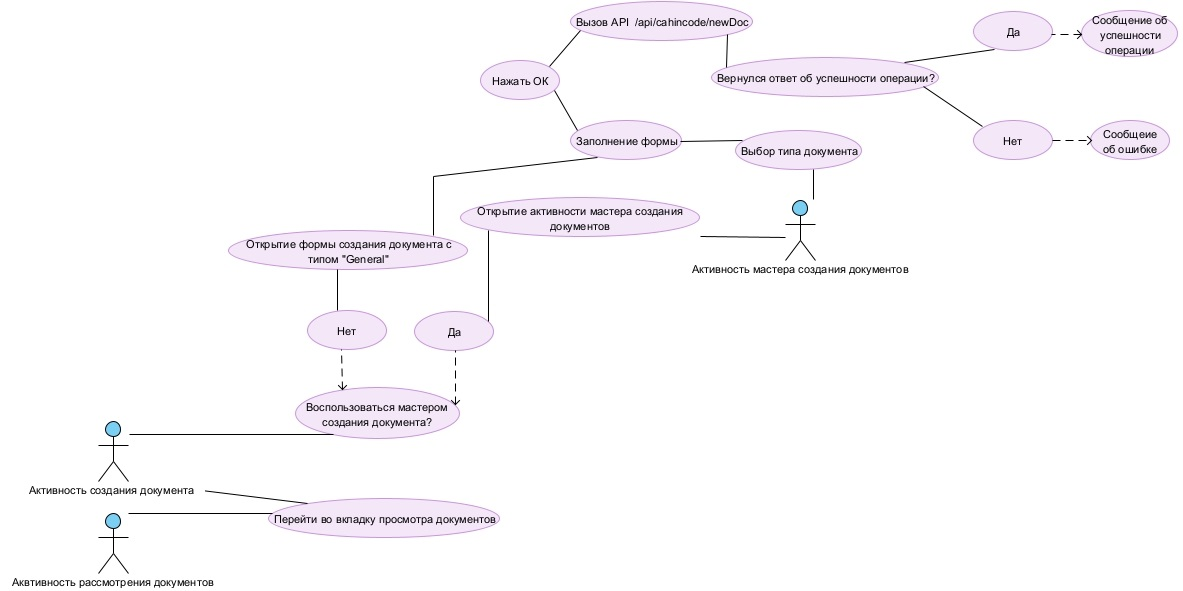
\includegraphics [scale=0.8] {CreateDocDiagram}
	\caption{Создание документов с использованием мастера и без.}
	\label{fig:user-scenario-create-doc}
\end{figure}
\begin{figure}[H]
	\centering
	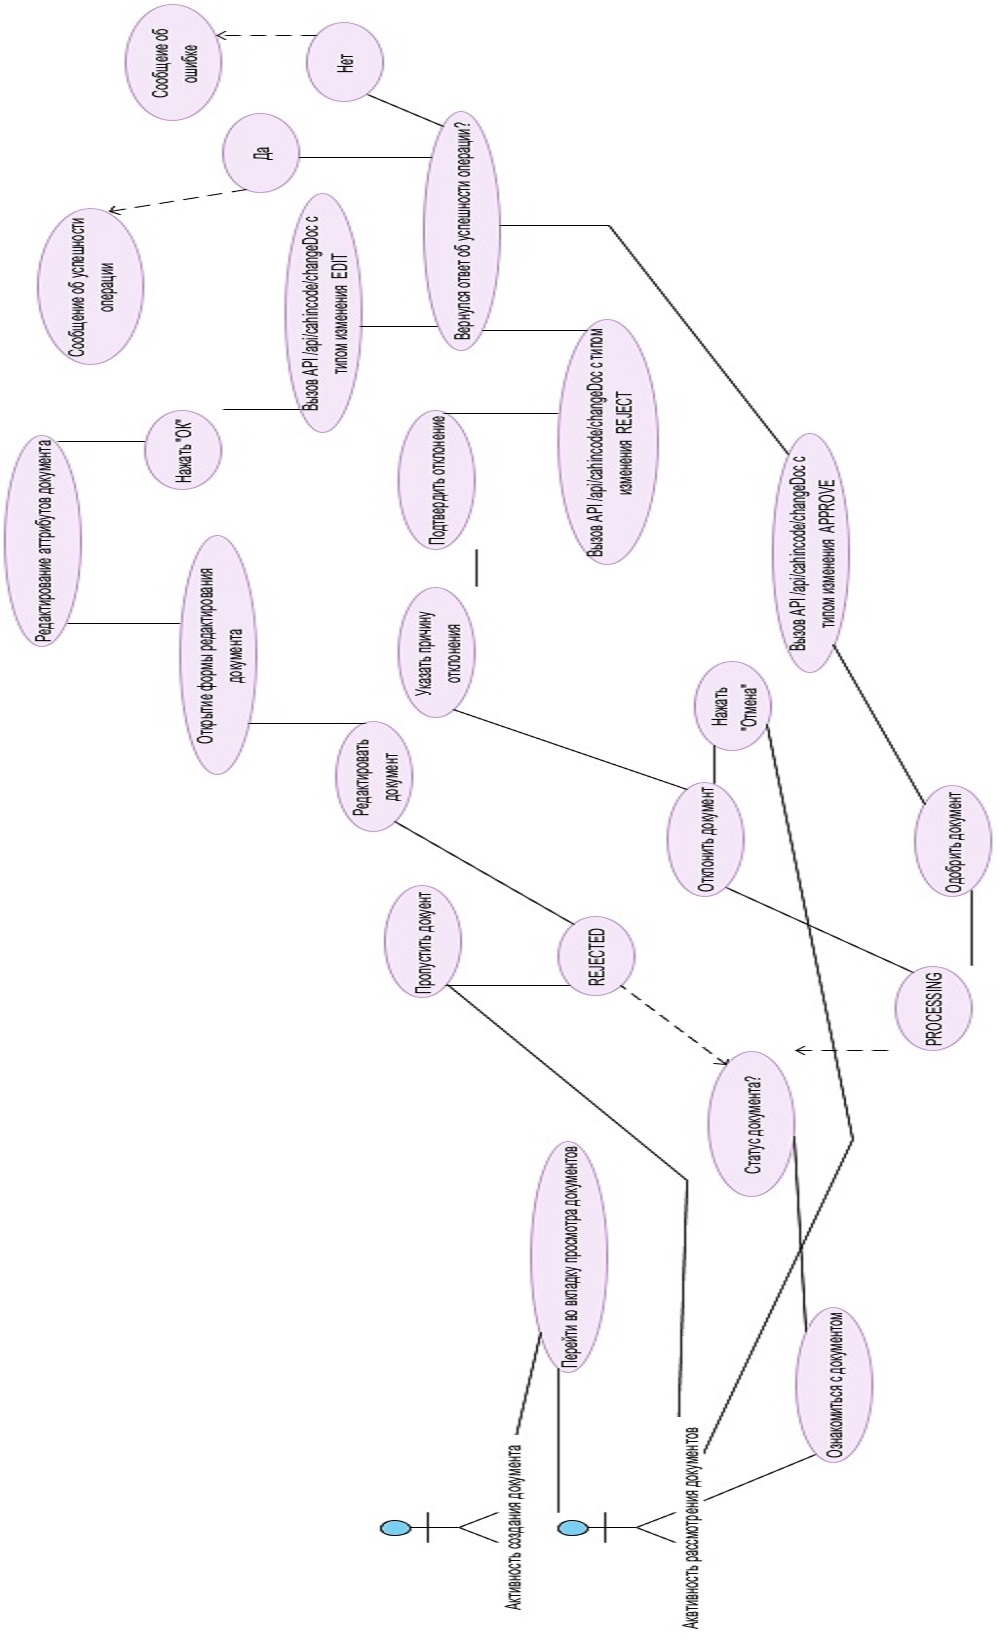
\includegraphics [scale=0.6] {ChangeDocDiagramRotated}
	\caption{Редактирование существующего документа.}
	\label{fig:user-scenario-last}
\end{figure}

С каждой активности, представленной на рисунках~\ref{fig:user-scenario-first}-\ref{fig:user-scenario-last}, за исключением активности аутентификации возможен переход к любой другой активности (за исключением, опять же, активности аутентификации) посредство навигационного меню, всегда находящегося под рукой пользователя. Такое меню является отличительным элементом многих мобильных приложений и играет не последнюю роль в вопросе <<юзабилити>>\cite{usability}.


 
